\newpage

\section{Вычислительный эксперимент}

\subsection{Модель автоследования} 

Автоследование --- способ инвестирования, при котором все желающие могут подключиться к стратегии более опытного инвестора (он же автор стратегии) и автоматически повторять все его сделки на своем счете. 

Для создания модели автоследования выделяются инвесторы - авторы стратегий автоследования Тинькофф инвестиций. 
\[\text{Ответ инвестора} = \frac{\text{Сумма сделки}}{\text{Объем портфеля}}\]

Путем усреднения ответов инвесторов о продаже или покупке акций составляется временной ряд $a_{0}, ..., a_{N}, a_{i} \in [-1, 1]$.

\begin{figure}[h!t]\center
{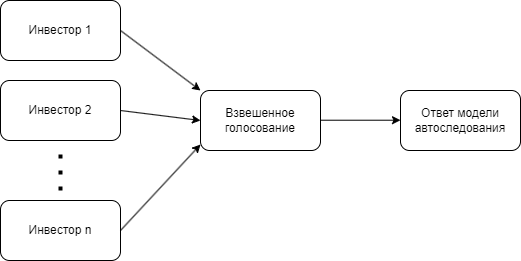
\includegraphics[width=0.8\textwidth]{results/voting.png}}
\caption{Модель автоследования}
\end{figure}

\subsection{Подготовка данных} 
Эксперимент проводится для временного ряда курса акций YNDX. 

Ряд приводится к стационарному виду следующими преобразованиями: \\
1) Дифференцирование: $y'_{t} = y_{t} - y_{t-1}$ \\ 
2) Сезонное дифференцирование $y' '_{t} = y'_{t} - y'_{t-s}, \ s=5$ \\

\begin{figure}[h!t]\center
\subfloat[]
{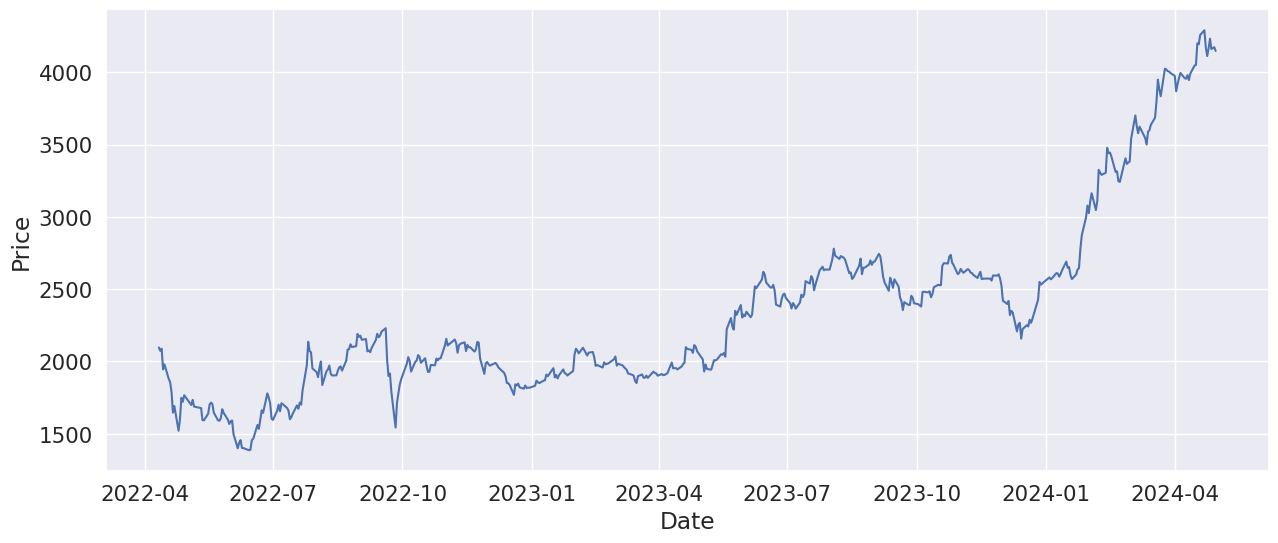
\includegraphics[width=0.5\textwidth]{results/yndx.png}}
\subfloat[]
{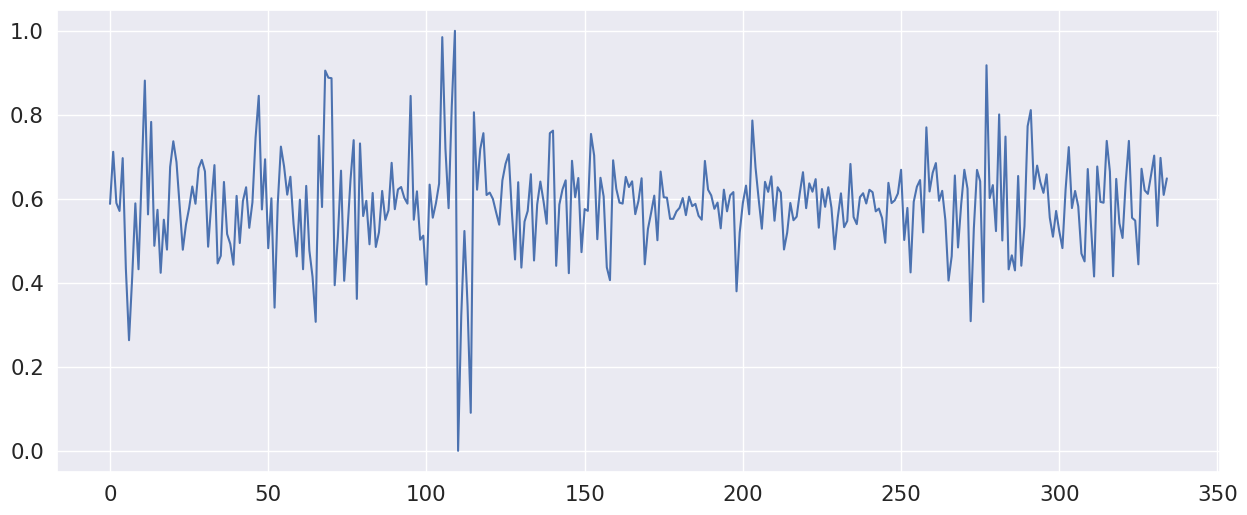
\includegraphics[width=0.5\textwidth]{results/yndx_stationary.png}}\\
\caption{Временной ряд курса акций YNDX до и после преобразований}
\end{figure}

Для проверки ряда на стационарность используется критерий KPSS: \\
Для исходного ряда $p-value < 0.01$ \\
Для полученного ряда $p-value > 0.01$ \\

\begin{figure}[h!t]\center
{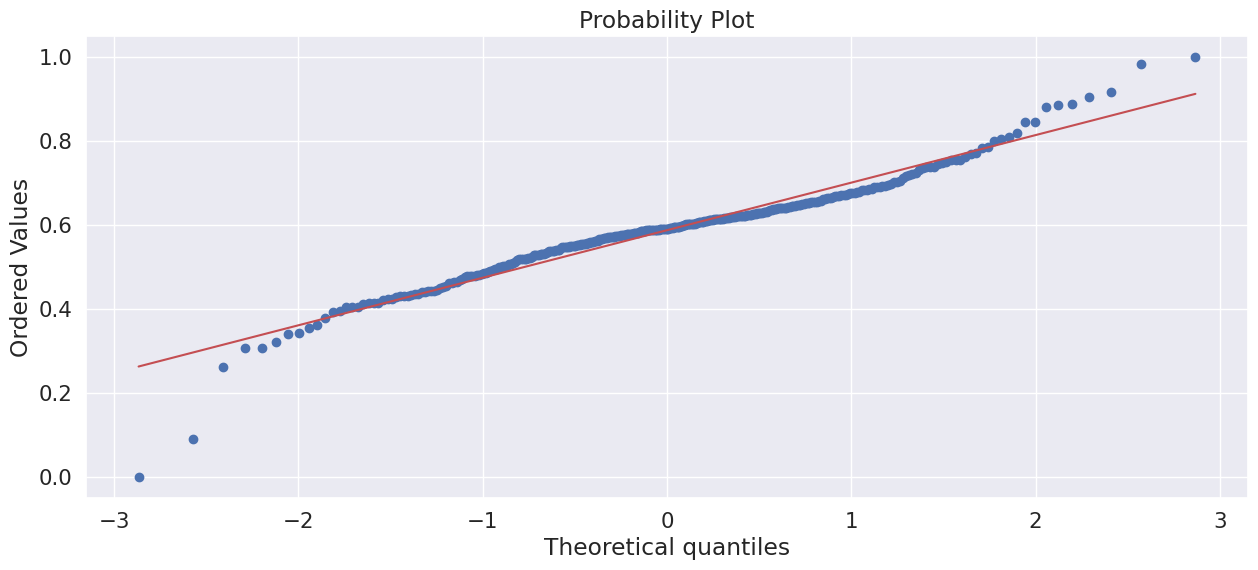
\includegraphics[width=0.8\textwidth]{results/qqplot.png}}
\caption{Q-Q plot полученного ряда}
\end{figure}

\begin{figure}[h!t]\center
{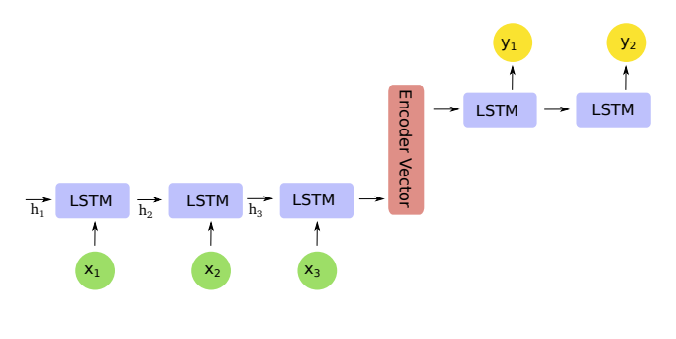
\includegraphics[width=0.8\textwidth]{results/seq2seq.png}}
\caption{sequence-to-sequence архитектура}
\end{figure}

\begin{table}[h!t]
\begin{center}
\caption{Выборки}
\label{table_2}
\begin{tabular}{|c|c|}
\hline
	Выборка & Пояснение \\
	\hline
	\multicolumn{1}{|l|}{YNDX-Train}
	& Обучающая часть \\
	\hline
	\multicolumn{1}{|l|}{YNDX-Test}
	& Тестовая часть \\
	\hline
	\multicolumn{1}{|l|}{TMOS-Train}
	& Обучающая часть \\
	\hline
	\multicolumn{1}{|l|}{TMOS-Test}
	& Тестовая часть \\
\hline

\end{tabular}
\end{center}
\end{table}


\subsection{Нахождение оптимального размера окна}

Для формирования обучающей выборки используется метод скользящего окна. 
Сравнение качества базовой модели на тестовой выборке в завимости от размера окна.


\subsection{Анализ качества модели прогнозирования}

В качестве базовой модели для задачи прогнозирования используется seq2seq архитектура на основе LSTM модели. При этом метод пресказания - рекурсивный.

Сравнение качества базовой модели на тестовой выборке в зависимости от использования ответов модели автоследования.

\begin{figure}[h!t]\center
{\includegraphics[width=0.8\textwidth]{results/loss_forecasting.png}}
\caption{Качество прогнозирования на тестовой выборке. Все результаты усреднены по 5 запускам}
\end{figure}

На рис. показан график зависимости средней кварадтичной ошибки на отложенной тестовой выборке между истинными значениями ряда и ответами модели.

\begin{figure}[h!t]\center
\subfloat[]
{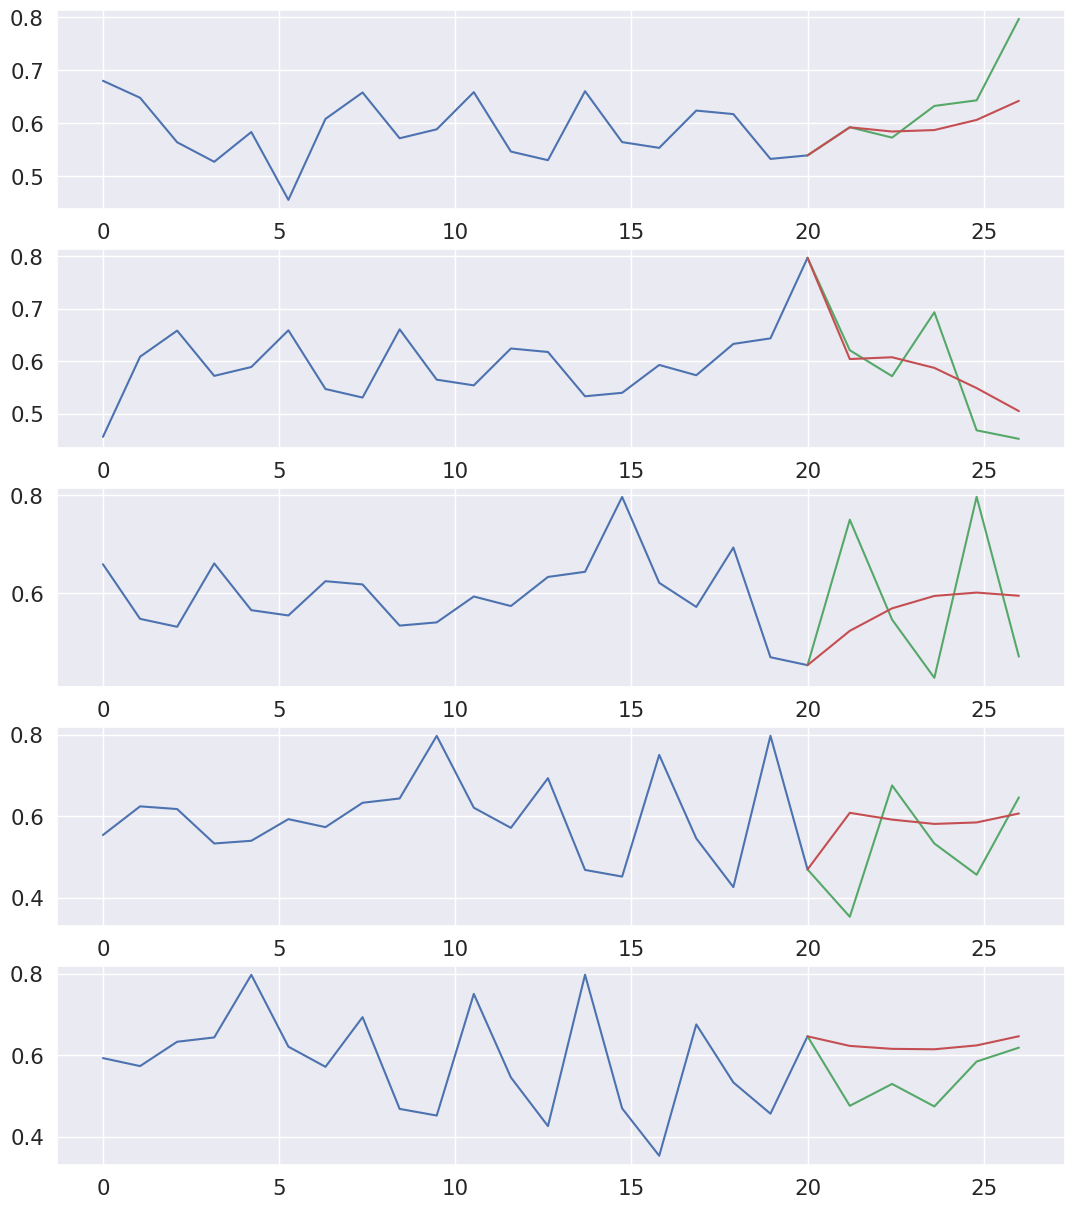
\includegraphics[width=0.5\textwidth]{results/forecasting_example_base.png}}
\subfloat[]
{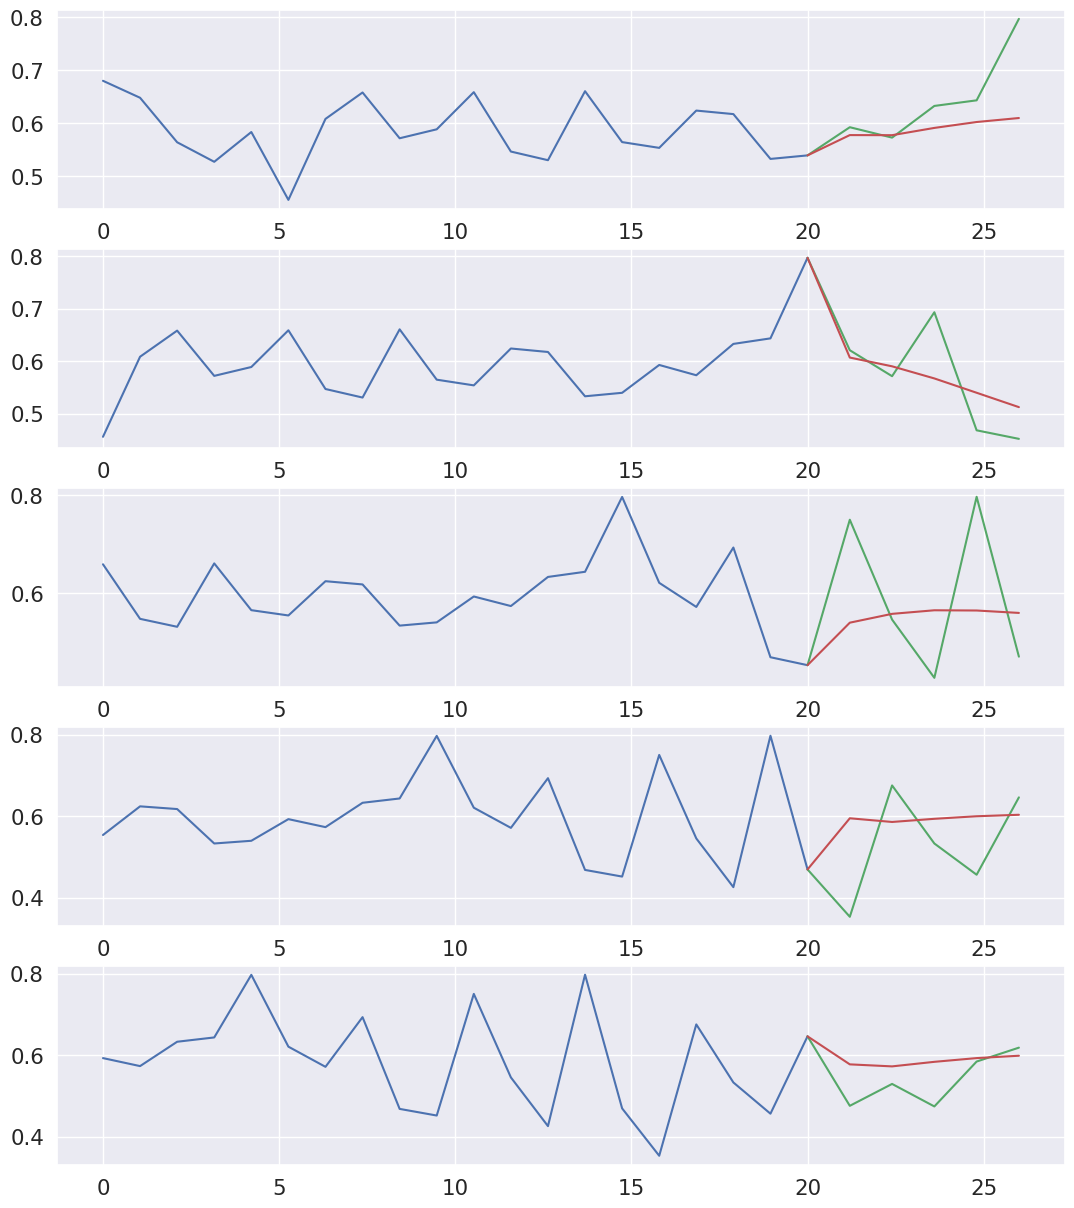
\includegraphics[width=0.5\textwidth]{results/forecasting_example_auto.png}}\\
\caption{Сравнение результатов прогнозирования. a) Без использования модели автоследования; b) С использованием модели автоследования}
\end{figure}

На рис. показаны примеры прогнозирования базовой модели на отложенной тесовой выборке.

На графиках видно, что модель, использующая ответы модели автоследования, показывает лучшее качество прогнозирования, при этом наблюдается снижение средней квадратичной ошибки. 

\subsection{Код вычислительного эксперимента}

Весь код вычислительного эксперимента представлен в~\cite{Github}. Также доступны письменный отчет и результаты экспериментов.